\chapter{Infraestructura}\label{cap.infraestructura}
\hspace{1cm} Una vez vistos los objetivos de este trabajo, en este capítulo se mostrarán las diferentes infraestructuras en las que nos hemos apoyado para la programación de la aplicación robótica de este TFG. También se explicará el funcionamiento de algunos componentes previos que hemos integrado.

\section{Gazebo}
\hspace{1cm} El simulador Gazebo es un programa \textit{OpenSource} distribuido bajo la licencia Apache 2.0 que se utiliza para investigación en robótica e Inteligencia Artificial.

\hspace{1cm} Este simulador ofrece la capacidad de simular de una forma eficiente y precisa cualquier tipo de robot en entornos complejos tanto de exterior como de interior. Sus características principales son sus motores de físicas, el motor de renderizado avanzado, el repositorio con la mayoría de robots comerciales y una gran gama de sensores y cámaras que permiten simular la mayoría de entornos reales.

\hspace{1cm} Al tratarse de un programa \textit{OpenSource} su comunidad crece a diario, lo que permite que cada vez existan más plugins, esto unido a la fácil integración en ROS e ICE permite que podamos tener el software base para simular los robots reales.
\\

\begin{figure}[H]
	\begin{center}
		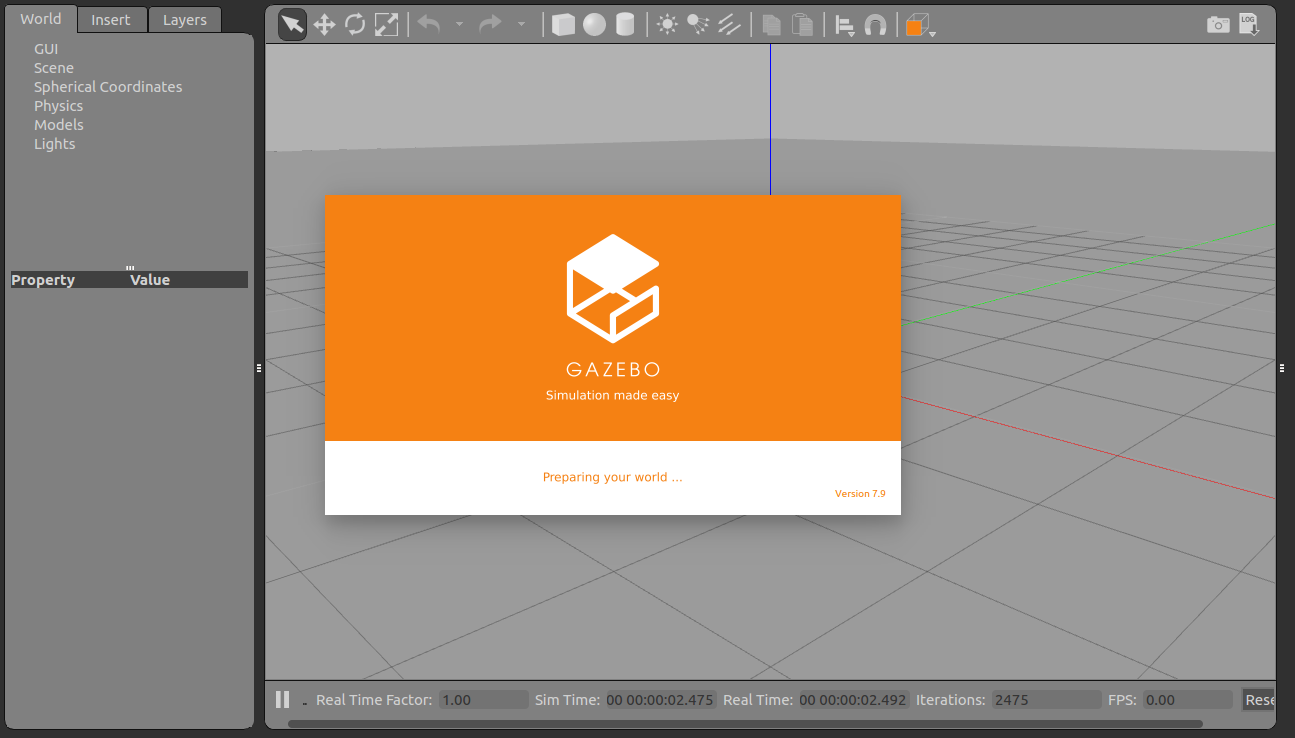
\includegraphics[width=1\textwidth]{imag/IMG18.png}
				\caption{Entorno de Simulación Gazebo.} 
	\label{fig:Gazebo.}	
	\end{center}
\end{figure}

\hspace{1cm} En este TFG se ha utilizado para simular al dron en un escenario con balizas y se ha programado la navegación autónoma de ese dron simulado, para ello se ha trabajado con la versión Gazebo 7.9. Los mundos creados en esta aplicación se pueden lanzar sin GUI o con GUI y se definen con la extensión '.world' y escritos mediante SDF \textit{(Simulation Description Format)}.

\section{Balizas visuales AprilTags}
\hspace{1cm} AprilTags \cite{AprilTags2} es una biblioteca para el sistema de visión por computador que permite detectar balizas visuales contenidas en una imagen. Es útil en una amplia variedad de tareas que incluyen la realidad aumentada, la robótica y la calibración de cámaras.

\hspace{1cm} Las balizas se basan en el concepto de los códigos QR, aunque éstas están diseñadas para contener muchos menos bits de información (4-12 bits). Además, presenta un nuevo sistema de codificación que aborda problemas específicos de los códigos de barras 2D como es la robustez frente a la rotación y a los falsos positivos que pueden dar las imágenes naturales. El software de detección AprilTag calcula la posición, orientación e identidad 3D precisa de las etiquetas en relación con la cámara, además de su correspondiente ID. Eso lo realiza mediante un algoritmo de segmentación basado en gradientes locales que consigue que las líneas se estimen con precisión, el cual se implementa en C sin dependencias externas. Esto provoca una tasa de falsos negativos muy bajos, aunque aumenta la probabilidad de falsos positivos. Sin embargo, gracias a la codificación de las balizas esta probabilidad es reducida hasta niveles aceptables.
\\

\begin{figure}[H]
	\begin{center}
		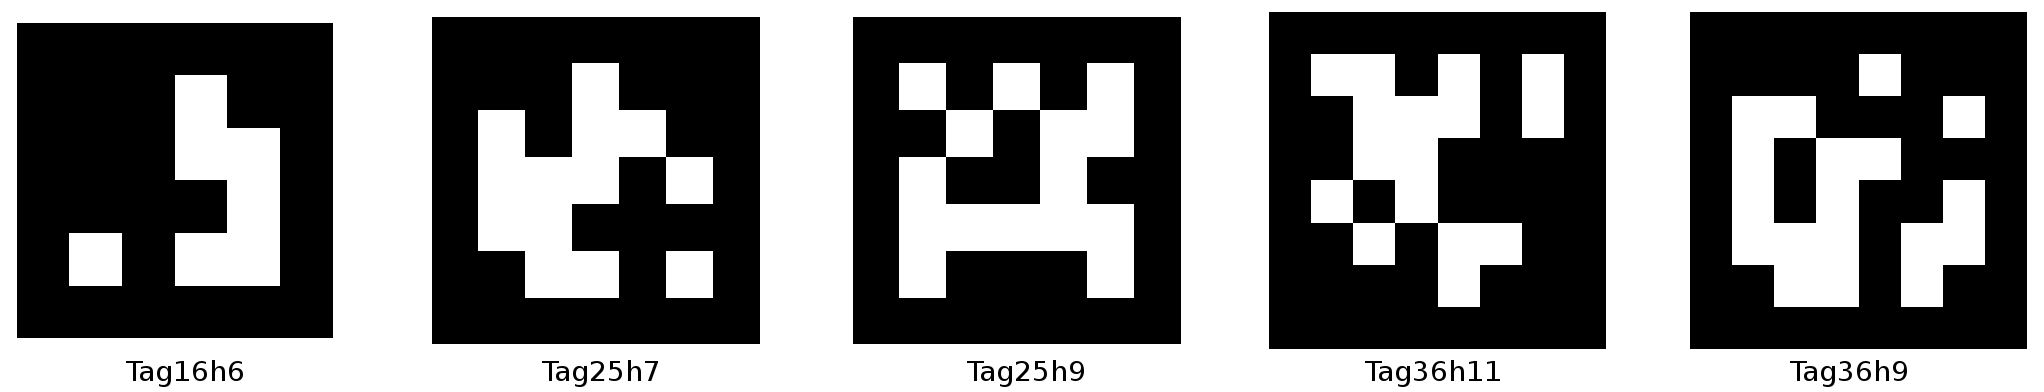
\includegraphics[width=0.8\textwidth]{imag/IMG25.png}
				\caption{Ejemplos de AprilTags.} 
	\label{fig:AprilTags.}	
	\end{center}
\end{figure}

\hspace{1cm} Esta biblioteca la hemos utilizado como ayuda al sistema de autolocalización de Slam-VisualMarkers y el código en C++ (que fue desarrollado primero por Edwin Olson y posteriormente por Michael Kaess) se puede obtener gratuitamente en su página \footnote{\url{http://people.csail.mit.edu/kaess/apriltags/}}, nosotros hemos utilizado su versión 2.1 dentro del componente de localización de Slam Visual-Markers.

\section{Biblioteca OpenCV}
\hspace{1cm} OpenCV \footnote{\url{https://opencv.org/}} es una biblioteca \textit{OpenSource} de visión artificial que se desarrolló inicialmente por Intel, tiene un conjunto de funciones que van desde sistemas de seguridad con detección de movimiento hasta centros de procesamiento con reconocimiento de objetos. Está programada en C/C++ y en nuestro TFG para el procesamiento de imágenes nos hemos apoyado principalmente sobre ésta, trabajando en la versión 3.4. 

\hspace{1cm} Gracias a OpenCV, al obtener la imagen que transmite el dron se puede tanto detectar objetos como aplicar cambios sobre ella, para marcar las zonas de interés o diferentes objetos. Permite la realización de filtros de color, por ejemplo para eliminar objetos no deseados dependiendo el momento. Además permite el uso de operadores morfológicos (erosión y dilatación) gracias a los cuales se evitan imperfecciones en las imágenes como ruidos, que confunde objetos inexistentes o de no interés con objetos de interés. En nuestro caso, nos ha servido tanto para la localización de las balizas de despegue y aterrizaje, como para la clasificación de las balizas AprilTags según la distancia a la que se encuentran del dron y por tanto el peso que tienen a la hora de estimar la posición.
\\

\begin{figure}[H]
	\begin{center}
		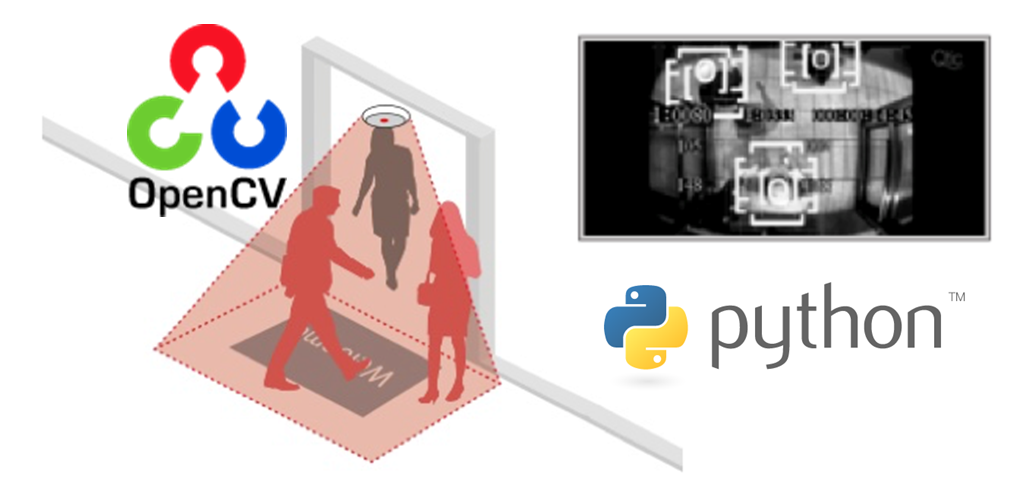
\includegraphics[width=0.8\textwidth]{imag/IMG26.png}
				\caption{Ejemplo de algoritmo con OpenCV.} 
	\label{fig:OpenCV.}	
	\end{center}
\end{figure}

\section{Biblioteca NumPy}
\hspace{1cm} Este TFG está escrito principalmente en el lenguaje de programación Python y NumPy \footnote{\url{http://www.numpy.org/}} es una extensión \textit{open-source} de este lenguaje. Es el paquete fundamental para la informática científica con Python. Contiene, entre otras cosas, un poderoso objeto de matriz N-dimensional, herramientas para integrar el código C/C++ y Fortran, álgebra lineal útil, transformadas de Fourier y capacidad de trabajo sobre números aleatorios. Concretamente en este TFG se ha utilizado la versión Py3.5.

\hspace{1cm} Además de sus usos científicos obvios, NumPy también se puede usar como un contenedor multidimensional de datos genéricos. A su vez se pueden definir tipos de datos arbitrarios, lo que permite a NumPy integrarse de manera rápida y sin problemas con una amplia variedad de bases de datos. NumPy está licenciado bajo la licencia BSD \textit{(Berkeley Software Distribution)}, lo que permite su reutilización con pocas restricciones.

\section{Entorno JdeRobot}
\hspace{1cm} JdeRobot \footnote{\url{http://jderobot.org/Main_Page}} es un paquete de software libre para desarrollar aplicaciones de robótica y visión por computación. Estas aplicaciones incluyen sensores como cámaras, actuadores y software inteligente en el medio. Está escrito principalmente en los lenguajes C++ y Python, y proporciona un entorno de programación basado en componentes. Pueden ejecutarse en diferentes ordenadores y se conectan mediante el \textit{middleware} de comunicación ICE o los mensajes ROS. Los componentes interoperan a través de interfaces explícitas. Es el software principal con el que hemos trabajado y está mantenido por el grupo de robótica de la Universidad Rey Juan Carlos.

\hspace{1cm} Para nuestro trabajo hemos utilizado la versión más reciente del repositorio, JdeRobot-5.6.3(Febrero 2018) \footnote{\url{https://jderobot.org/Installation}}. Nos ha servido como herramienta para comprender los componentes previos que hemos utilizado y la aplicación final es un conjunto de nodos desarrollados en el ecosistema JdeRobot.

\subsection{Herramienta ColorTuner}
\hspace{1cm} Es una aplicación para configurar filtros de color personalizados en espacios de color HSV, RGB o YUV, y así obtener la gama de color que nos interesa o realizar un filtro sobre una imagen o vídeo. Utiliza un interfaz gráfico donde se representan dos imágenes, una la real y otra la filtrada, en ésta se pueden variar los parámetros para ver qué colores cumplen las características, quedándose los otros en negro. Se ha utilizado para extraer los colores de las balizas de aterrizaje y despegue y así poner su gama de colores correctamente en los filtros de la aplicación final para que el dron las encuentre sin problemas.

\begin{figure}[H]
	\begin{center}
		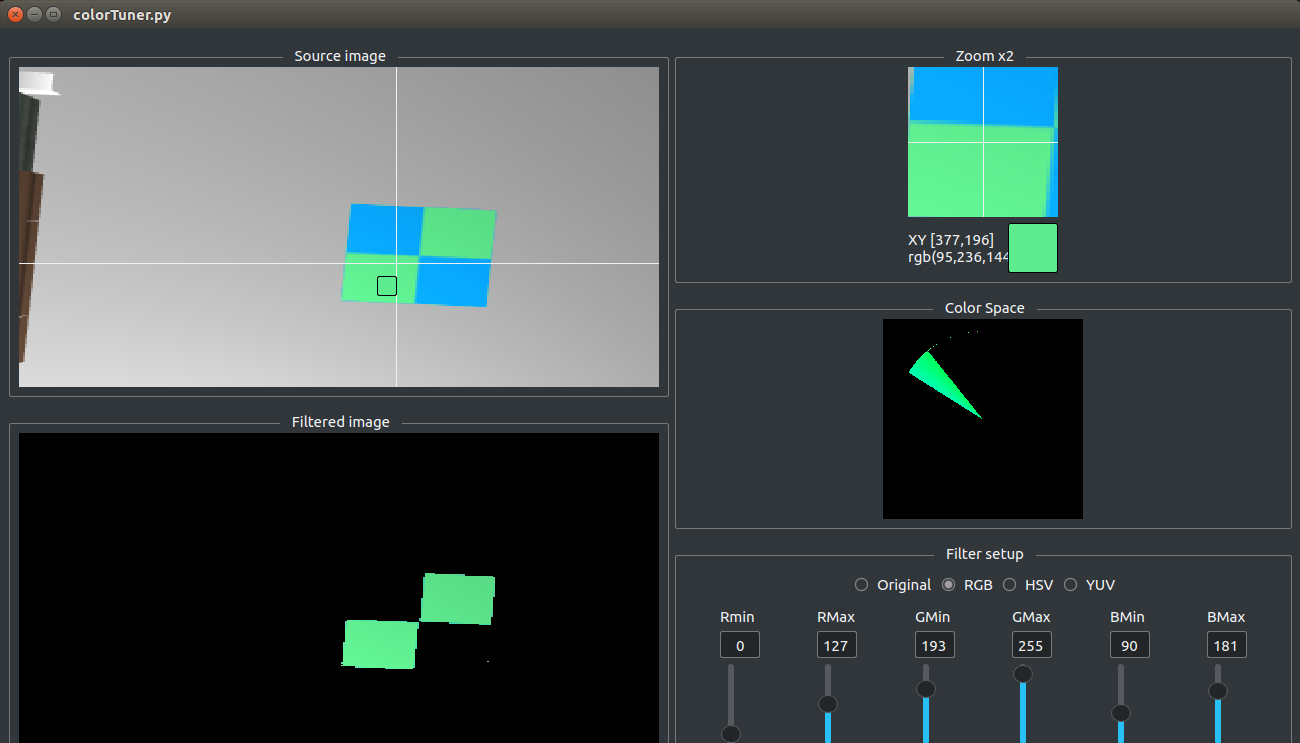
\includegraphics[width=1\textwidth]{imag/IMG27.png}
				\caption{Herramienta ColorTuner.} 
	\label{fig:ColorTuner.}	
	\end{center}
\end{figure}

\subsection{Plugin ArDrone2 en Gazebo}
\hspace{1cm} Hemos empleado para el desarrollo del proyecto el ArDrone 2.0 o más bien su modelo en el entorno de simulación Gazebo. Este plugin implementa una emulación realista y optimizada en simulación del dron, por lo que nos permite trabajar con los distintos sensores. Este dron cuenta con sensores IMU y con dos cámaras, una frontal y otra ventral, con ello el simulador Gazebo es capaz de ofrecer datos como la posición del dron o las imágenes que ve el mismo. También cuenta con una brújula, un altímetro y cuatro motores cada uno con su correspondiente hélice, lo que nos permite enviar al dron una serie de comandos mediante el interfaz \textit{CMDVel} para dirigir sus movimientos y saber en todo momento en qué posición se encuentra.

\subsection{Interfaz Pose3D}
\hspace{1cm} Pose3D es la interfaz que se emplea en JdeRobot para obtener la posición y orientación en un espacio 3D de un objeto, en nuestro caso un dron. Se implementa mediante la función \emph{Pose3Ddata} y está compuesta por un punto en 3D (el cual indica la posición en coordenadas cartesianas) y la orientación mediante los cuaterniones. A partir de éstos podremos obtener los ángulos de \textit{roll, pitch} y \textit{yaw}.

\begin{figure}[H]
 \centering
  \subfloat[Datos de Pose3DData]{
   \label{f:Pose3DData}
    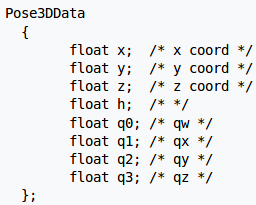
\includegraphics[width=0.25\textwidth]{imag/IMG20.png}}
  \subfloat[Representación de los datos]{
   \label{f:Datos}
    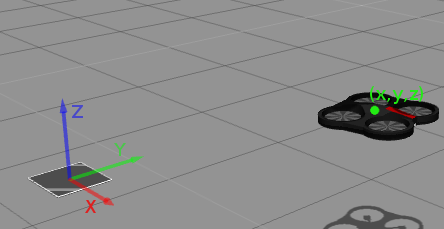
\includegraphics[width=0.35\textwidth]{imag/IMG21.png}} 
  \subfloat[Matriz de Conversión Angular]{
   \newline\label{f:Matriz Angular}
    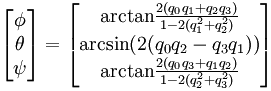
\includegraphics[width=0.35\textwidth]{imag/IMG22.png}} 
 \caption{Ejemplo de Pose3DData}
 \label{f:Ejemplo de Pose3DData}
\end{figure} 

\section{Visual States}
\hspace{1cm} VisualStates es una herramienta para la programación de comportamientos de robots que utilizan máquinas de estados finitos jerárquicas \textit{(HFSM - Hierarchichal Finite State Machine)}. Permite el diseño gráfico de la inteligencia de un robot expresándola como estados y transiciones, además genera automáticamente un nodo JdeRobot en Python que lo materializa. Representa el comportamiento del robot gráficamente en una hoja en blanco compuesto por estados y transiciones. Cuando el autómata está en un cierto estado, pasará a otro dependiendo de las condiciones establecidas en las transiciones. Esta representación gráfica permite un mayor nivel de abstracción para el usuario, ya que sólo tiene que preocuparse por programar las acciones actuales del robot y seleccionar qué componentes puede necesitar de la interfaz del robot.
\\
\\
\begin{figure}[H]
	\begin{center}
		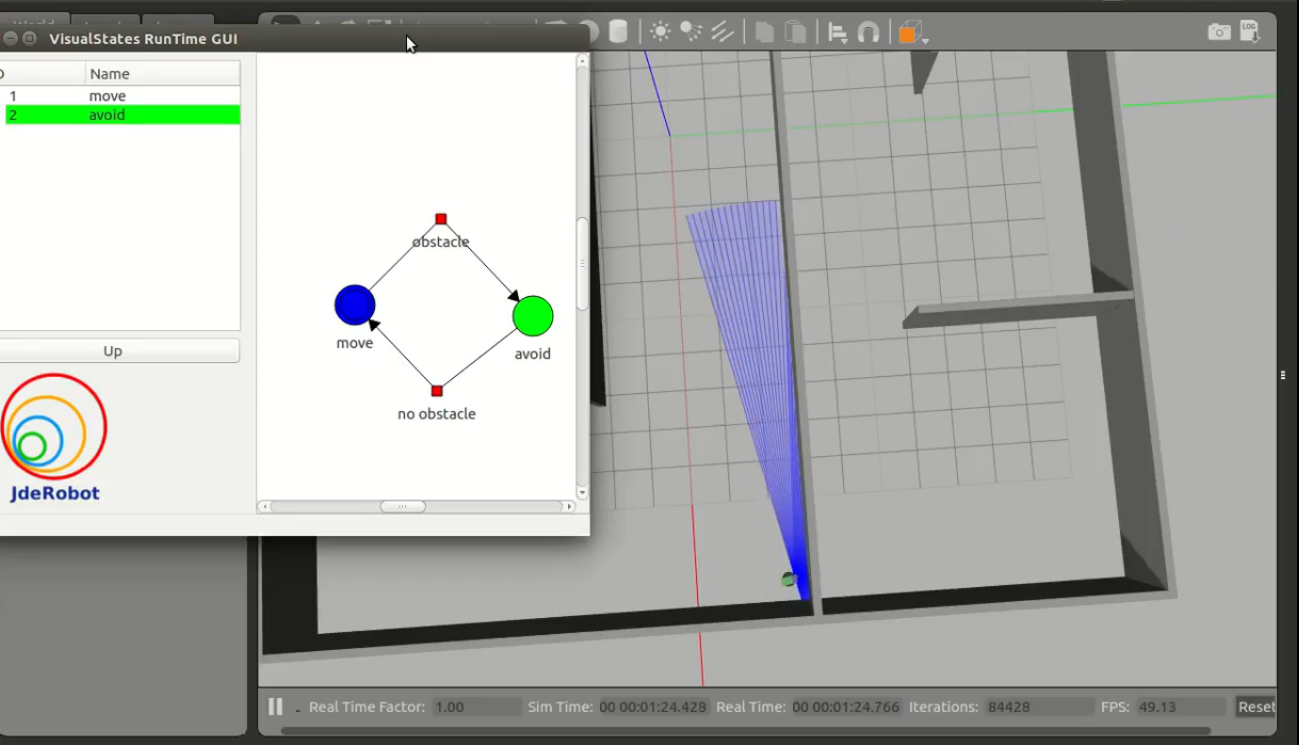
\includegraphics[width=1\textwidth]{imag/IMG19.png}
				\caption{Herramienta VisualStates sobre Gazebo} 
	\label{fig:Visual States.}	
	\end{center}
\end{figure}

\hspace{1cm} Esta herramienta cuenta con una interfaz de usuario, la cual varía según estemos modificando el código o ejecutándolo. La GUI de VisualStates permite el diseño de autómatas y la GUI de tiempo de ejecución de Python proporciona una visualización del autómata en ejecución. 

\hspace{1cm} En nuestro TFG hemos utilizado esta herramienta para la creación de nuestro propio autómata, gracias a ello hemos podido dividir el problema final en subapartados y solucionarlos poco a apoco hasta llegar al algoritmo final. Se puede encontrar una guía de la herramienta en la web \footnote{\url{https://jderobot.org/Tutorials\#VisualStates_tool}}.

\section{Slam-Visualmakers}
\hspace{1cm} Es un nodo disponible en el ecosistema de JdeRobot que mediante una serie de algoritmos localiza en 3D la cámara a partir de balizas visuales en la escena. Es una aplicación desarrollada por Felipe Pérez \footnote{\url{http://jderobot.org/Flperezz-tfm}} en su Trabajo Fin de Máster que ha ido creando paralelamente a este TFG. Está desarrollado en la plataforma JdeRobot y está programado en C++. 

\begin{figure}[H]
	\begin{center}
		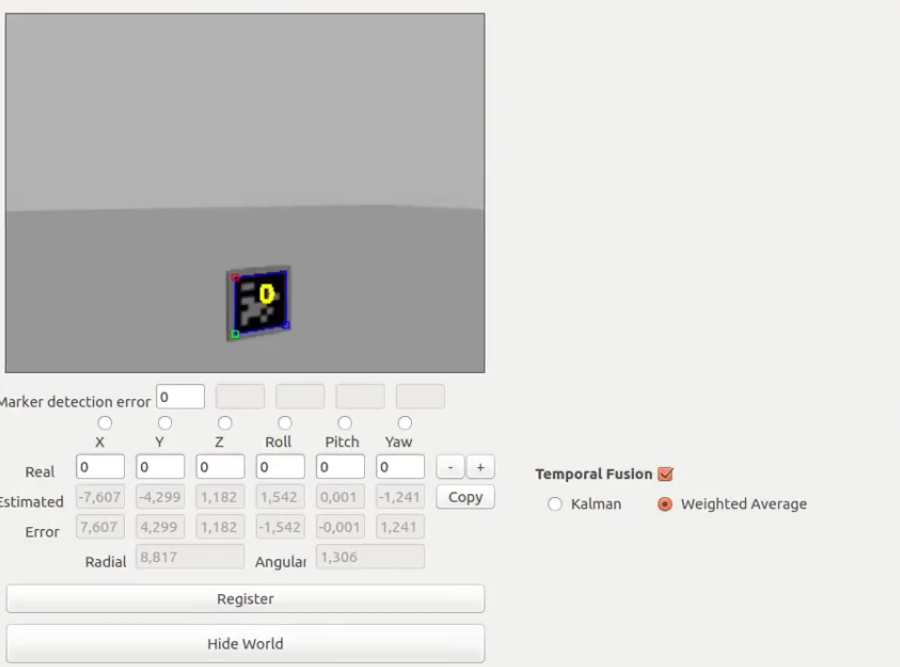
\includegraphics[width=0.55\textwidth]{imag/IMG24.png}
				\caption{GUI de Slam-Visualmarkers.} 
	\label{fig:GUI de Slam-Visualmarkers.}	
	\end{center}
\end{figure}

%\hspace{1cm} Esta aplicación es un desarrollo de Cam-Autoloc, pero con un algoritmo de estimación de posición más preciso, un interfaz gráfico propio, eliminando así la dependencia de QtCreator's, y la eliminación de la librería Aruco para su ejecución. 

\hspace{1cm} Para su correcto funcionamiento el algoritmo necesita tres entradas de datos: primero, se sirve de las imágenes recibidas a través de una interfaz creada con ICE y devuelve la posición estimada mediante un objeto Pose3D; segundo, un fichero de texto que contiene una lista donde figuran el identificador, posición y orientación 3D absolutas de cada baliza visual ubicada en el entorno; y tercero, un fichero de configuración que contiene toda la información de los parámetros ópticos de la cámara utilizada. 

\hspace{1cm} Para estimar la posición el algoritmo comienza analizando la imagen recibida mediante las librerías OpenCV y AprilTags para explorar la imagen en 2D en busca de las balizas. Una vez localizadas, se hace uso de la librería Progeo y la función SolvePnP de OpenCV para calcular la posición y orientación en tres dimensiones de la cámara con respecto a cada marcador. Finalmente, se realiza un proceso de fusión temporal y fusión espacial de la estimación obtenida a partir de cada baliza detectada en la imagen. La aplicación permite elegir qué clase de filtro temporal utilizar, pudiendo escoger entre un filtro por pesos o un filtro Kalman.

\begin{figure}[H]
	\begin{center}
		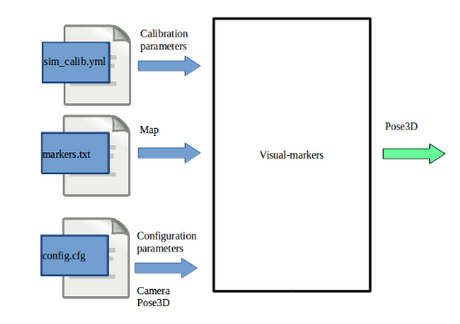
\includegraphics[width=0.8\textwidth]{imag/IMG23.png}
				\caption{Entradas y Salidas del nodo Slam-VisualMarkers.} 
	\label{fig:Entradas y Salidas del nodo.}	
	\end{center}
\end{figure}
